\documentclass[a4paper]{article}
\usepackage[top=0cm, bottom=0cm, left=0cm, right=0cm]{geometry}
\usepackage{tikz}
\usepackage{hyperref}
\usepackage{marvosym}
\usepackage[utf8]{inputenc}
\usetikzlibrary{patterns}
\usetikzlibrary{shapes,arrows}
\usetikzlibrary{decorations.pathreplacing, positioning}
\definecolor{anti-flashwhite}{rgb}{0.95, 0.95, 0.96}


\begin{document}
\noindent
  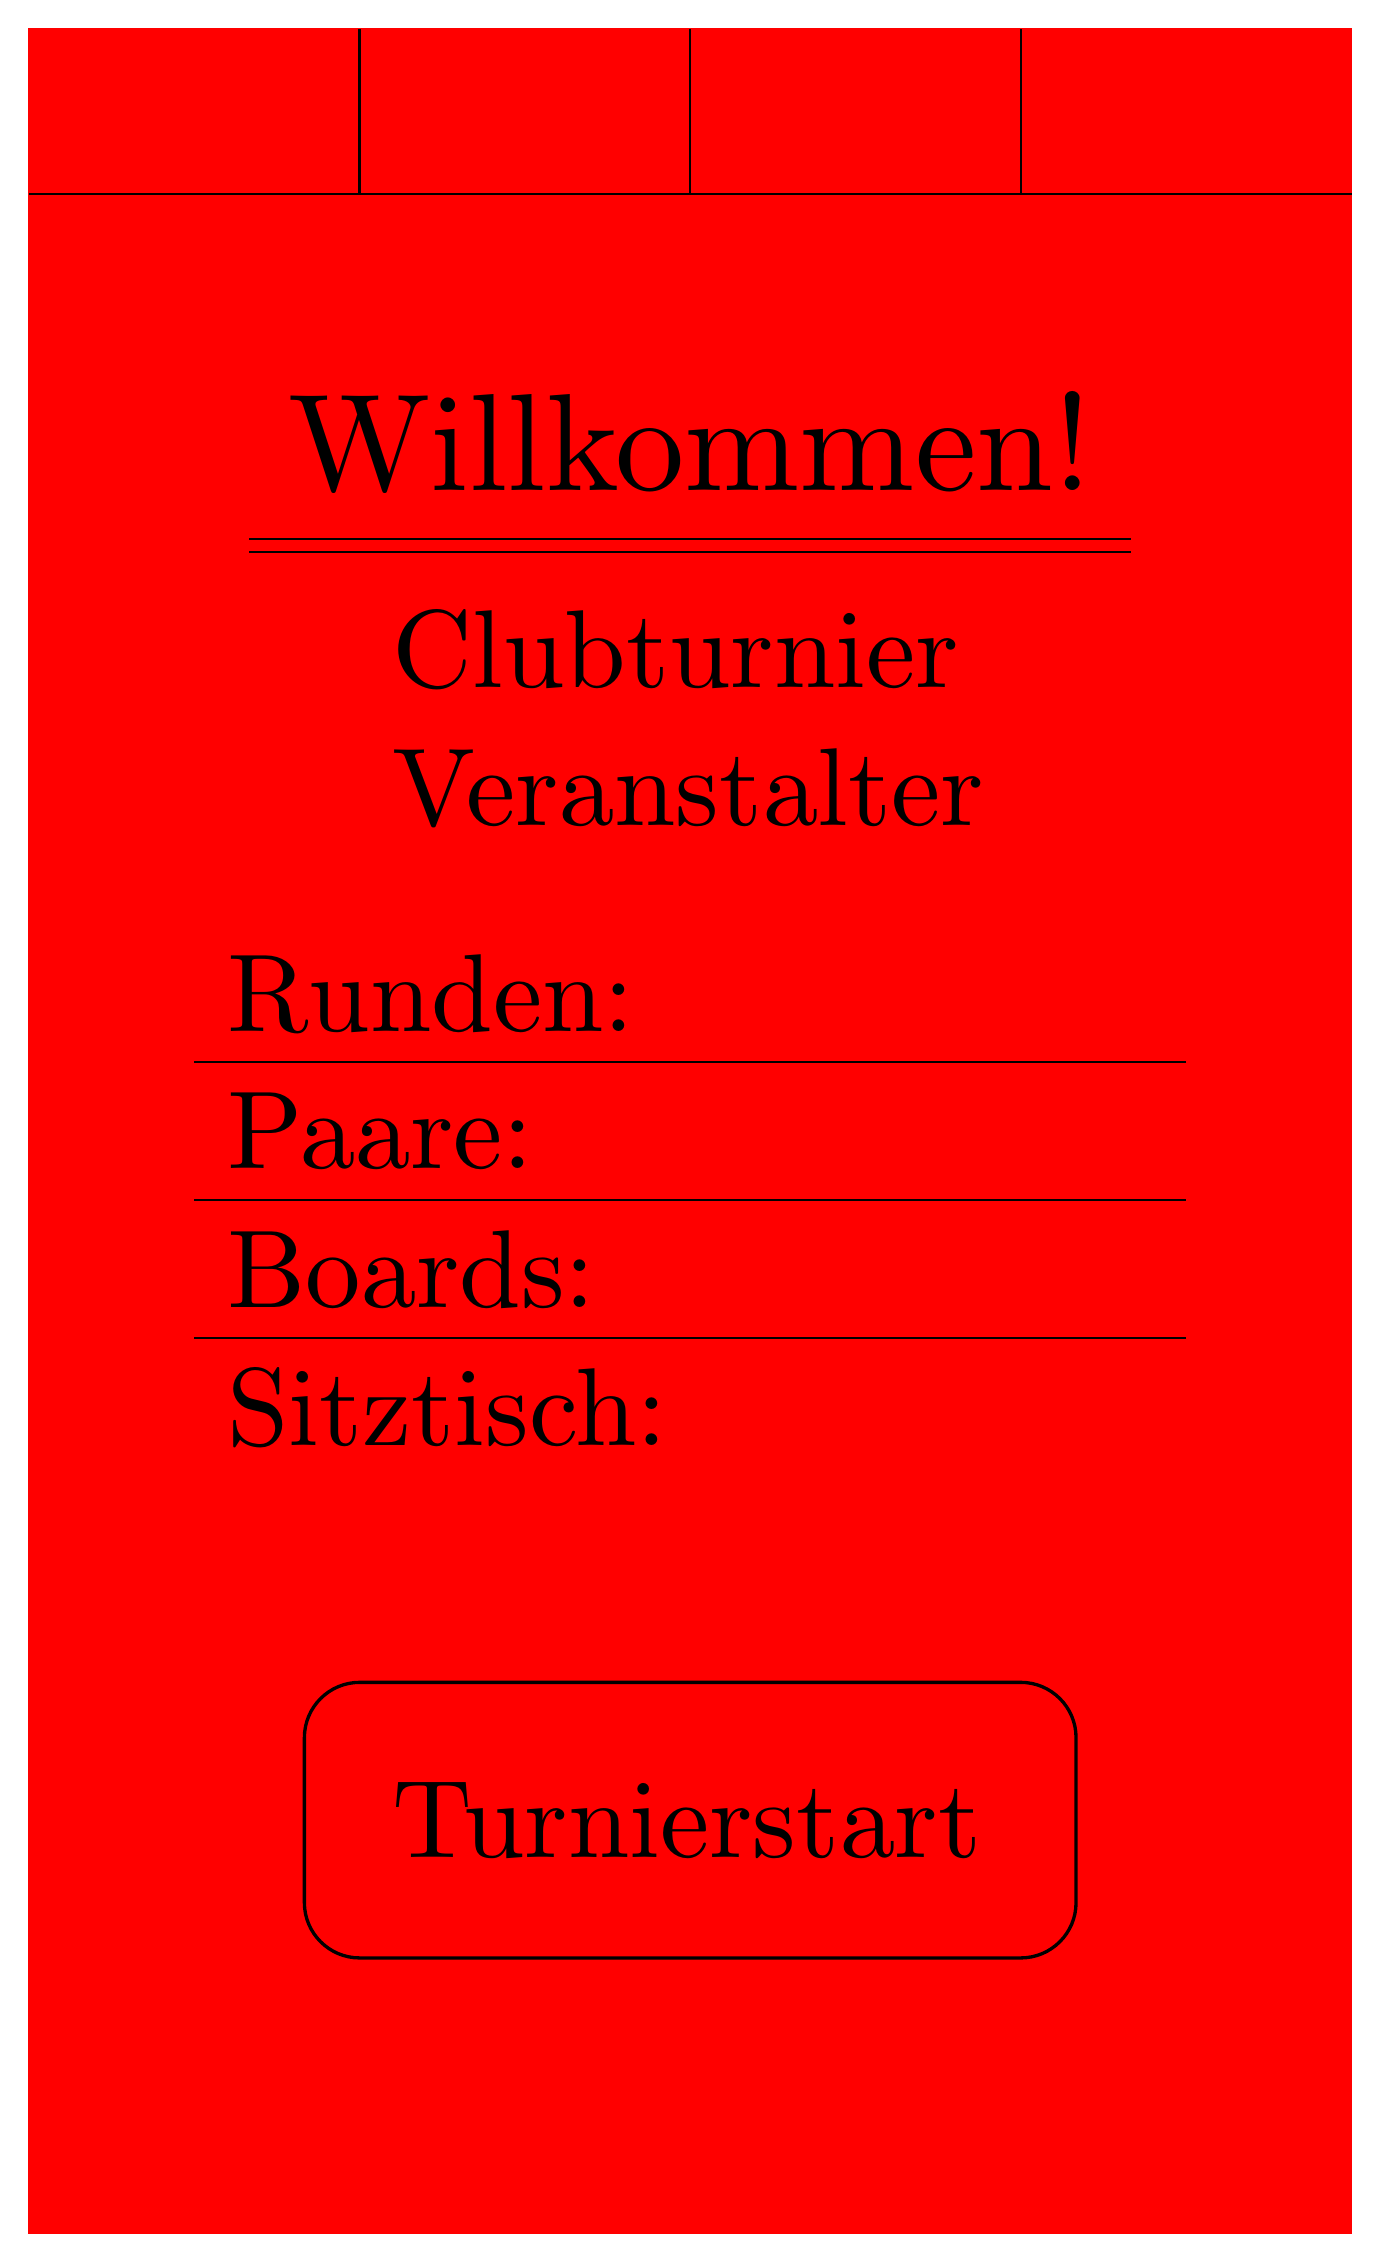
\begin{tikzpicture}[scale=0.35]
    % Background
    \draw[fill=white, color=red!!20] (48,80) -- (0,80) -- (0, 0) -- (48, 0) -- cycle;

    \draw[thick] (0, 74) -- (48, 74);
\foreach \x in {12, 24, 36}
  \draw[thick] (0 + \x, 80) -- (0 + \x, 74);


    \node[thick, align=center, scale=5] at (24, 65) {Willkommen!};
    \draw[thick] (8, 61) -- (40, 61);
    \draw[thick] (8, 61.5) -- (40, 61.5);

    \node[thick, align=center, scale=4, text width=4] at (14, 57.5) {Clubturnier};
    \node[thick, align=center, scale=4, text width=4] at (14, 52.5) {Veranstalter};

    \node[thick, align=left, scale=4, text width=4] at (8, 45) {Runden:};
    \draw[thick] (6, 42.5) -- (42, 42.5);
    \node[thick, align=left, scale=4, text width=4] at (8, 40) {Paare:};
    \draw[thick] (6, 37.5) -- (42, 37.5);
    \node[thick, align=left, scale=4, text width=4] at (8, 35) {Boards:};
    \draw[thick] (6, 32.5) -- (42, 32.5);
    \node[thick, align=left, scale=4, text width=4] at (8, 30) {Sitztisch:};

    \draw[very thick, rounded corners=20] (10, 20) -- (38, 20) -- (38, 10) -- (10, 10) -- cycle;

    \node[thick, align=center, scale=4, text width=4] at (14, 15) {Turnierstart};


  \end{tikzpicture}
\end{document}
